\documentclass[12pt]{article}

% Layout.
\usepackage[top=1in, bottom=0.75in, left=1in, right=1in, headheight=1in, headsep=6pt]{geometry}

% Fonts.
\usepackage{mathptmx}
\usepackage[scaled=0.86]{helvet}
\renewcommand{\emph}[1]{\textsf{\textbf{#1}}}

% TiKZ.
\usepackage{tikz, pgfplots}
\usetikzlibrary{calc}

% Misc packages.
\usepackage{amsmath,amssymb,latexsym}
\usepackage{graphicx}
\usepackage{array}
\usepackage{xcolor}
\usepackage{multicol}
\usepackage{fancyhdr}
\pagestyle{fancy}


% Misc.
\renewcommand{\d}{\displaystyle}
\newcommand{\ds}{\displaystyle}
\newcommand{\ul}[1]{\underline{#1}}
\def\bc{\begin{center}}
\def\ec{\end{center}}
\def\be{\begin{enumerate}}
\def\ee{\end{enumerate}}

\newcommand{\ans}[1][1in]{\rule{#1}{.5pt}}


\lhead{Math F113X: Quiz 5}
\rhead{17 October, 2025}

\begin{document}

\vspace{1cm}

\noindent \textbf{Name:} \hrulefill \quad  score:\ans[1cm] \ / 10 \\


There are 10 points possible on this quiz. No aids (book, notes, etc.)
are permitted. You may use a non-programmable calculator.  {\bf Show all work and supporting calculations for full credit. Explain how you get your answers.}



\be

	\item (4 points) Recall Dijkstra's algorithm says the following:
	
	\fbox{Dijkstra's Algorithm}

\textbf{input:} a graph with distances (weights) on the edges and a starting vertex, say $s$\\
\textbf{output:} the shortest distance between $s$ and every vertex in the graph\\
\textbf{rough strategy:} All vertices get \emph{tentative} distances to vertex $s$. One-by-one, vertices are explored and tentative distances are updated until minimum distances are obtained. Break ties alphabetically.\\
%\textbf{Steps:}
%\begin{enumerate}
%	\item (Initialization Step) Set the tentative distance to be zero for $s$ and $\infty$ for all other vertices.
%	\item (Iterative Step) Find the vertex, say $x$, with the smallest tentative distance \textit{that has not already been explored}. (Break any ties alphabetically.)
%		\begin{enumerate} 
%		\item For every edge between $x$ and a vertex (say $y$) \textit{that has not already been explored}, calculate the sum of the distance to $x$ plus the distance along the edge to $y.$ If this sum is \emph{smaller} than the tentative distance at $y$, replace the tentative distance with the smaller value. Otherwise, leave the tentative distance of $y$ unchanged.
%		\item Mark $x$ as \emph{explored} and record its tentative distance to $s$ as its \emph{minimum} distance to $s.$
%		\item If $x$ is the last vertex then terminate the algorithm, otherwise return to the beginning of the iterative step.
%		\end{enumerate} 
%\end{enumerate}

	
	
Use {\bf Dijkstra's algorithm} to determine the distances between vertex $S$
and each other vertex. Clearly show the steps of the algorithm in the
space provided.
	
	\begin{center}
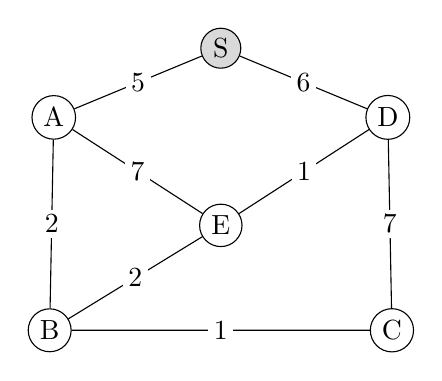
\begin{tikzpicture}[baseline=(current bounding box.center),lbl/.style={inner sep = 2pt, fill = white}, scale = 1.5]
\tikzstyle{vtx}=[circle, draw, inner sep=2pt]
\node[vtx, fill = gray!30] (S) at (90:2) {S};
\node[vtx] (A) at (135:2) {A};
\node[vtx] (B) at (45:2) {D};
\node[vtx] (D) at (90:0.5){E};
\node[vtx] (C) at (15+180:1.5){B};
\node[vtx] (E) at (-15:1.5){C};
\foreach \i/\j/\k in {S/A/5,S/B/6,A/C/2, A/D/7,B/D/1,B/E/7,C/E/1,C/D/2}{\draw (\i) --node[lbl]{\k} (\j);}
\end{tikzpicture}
\end{center}


\begin{minipage}[t]{.6\linewidth}
\vspace{0pt}
\begin{tabular}{ c | c | p{1.5in}}
Explored? & vertices & tentative distances\\ \hline
&S& \\[12pt] \hline
&A& \\[12pt]\hline
&B& \\[12pt]\hline
&C& \\[12pt]\hline
&D& \\[12pt]\hline
&E& \\[12pt]\hline
 \end{tabular}

 \end{minipage}
% 
%\vspace{1cm}
%
 %
 \begin{minipage}[t]{.4\linewidth}
 \vspace{0pt}
   List the vertices in the order you \\ explored them. \\
   \underline{\hspace{5.5cm}}
     \vspace{1cm}
     
     List the \emph{final} distances to $S$.
     
     \bigskip

\begin{tabular}{c || c | c | c | c | c | c}
vertex & $S$ & A &  B& C & D & E \\ \hline
distance from $S$ & &&&&& \\[12 pt]
\end{tabular}


 \end{minipage}
\vfill


\vfill


\newpage

\item (6 points) Consider the following graph.

\begin{center}
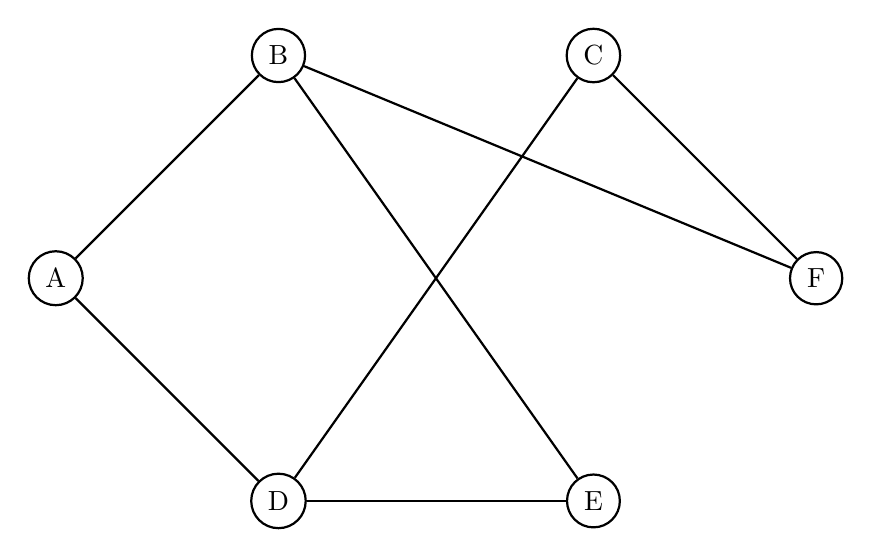
\begin{tikzpicture}[node distance={4cm}, thick, main/.style = {draw, circle}]
  \node[main] (1) {A};
  \node[main] (2) [above right of=1] {B};
  \node[main] (3) [right of=2] {C};
  \node[main] (4) [below right of=1] {D};
  \node[main] (5) [right of=4] {E};
  \node[main] (6) [below right of=3] {F};
  \draw (1) -- (2);
  \draw (1) -- (4);
  \draw (2) -- (5);
  \draw (2) -- (6);
  \draw (3) -- (4);
  \draw (3) -- (6);
  \draw (4) -- (5);
\end{tikzpicture}
\end{center}

\be
  \item Explain why this graph does not have an {\bf Euler
      circuit}.
    \vfill
    
  \item  Add additional edges to {\bf Eulerize} the graph
    above.
    \vspace{0.5cm}

  \item  Add the additional edges to the copy of the graph
    below and draw an {\bf Euler circuit} on the graph. Offset it slightly from the graph so the order it is traveled in is clear.
    
\begin{center}
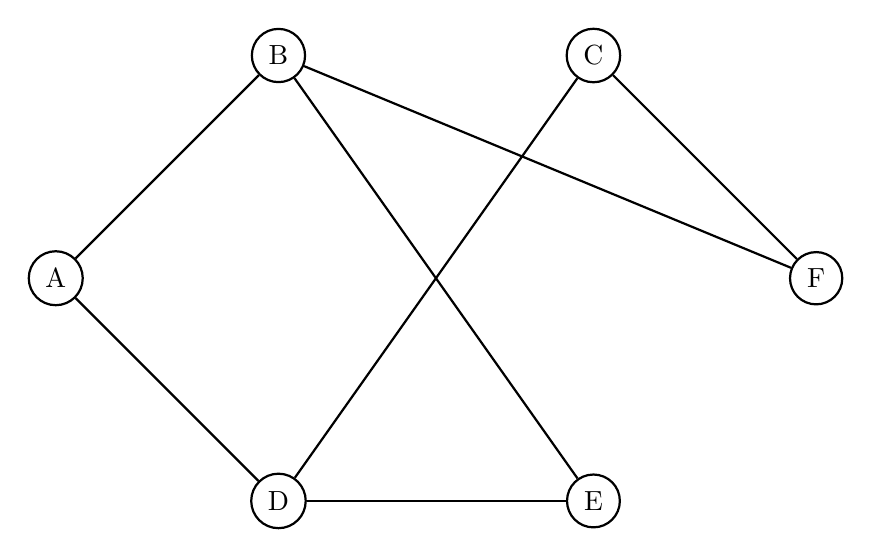
\begin{tikzpicture}[node distance={4cm}, thick, main/.style = {draw, circle}]
  \node[main] (1) {A};
  \node[main] (2) [above right of=1] {B};
  \node[main] (3) [right of=2] {C};
  \node[main] (4) [below right of=1] {D};
  \node[main] (5) [right of=4] {E};
  \node[main] (6) [below right of=3] {F};
  \draw (1) -- (2);
  \draw (1) -- (4);
  \draw (2) -- (5);
  \draw (2) -- (6);
  \draw (3) -- (4);
  \draw (3) -- (6);
  \draw (4) -- (5);
\end{tikzpicture}
\end{center}

\ee

% \item (3 points) Does the graph below contain an Euler circuit? An Euler path? You are \emph{not} asked to find one, only to determine if one exists. \emph{Justify your conclusion.}\\

% \begin{tikzpicture}[baseline=(current bounding box.center),scale=1.5]
% \tikzstyle{vertex}=[circle, draw, inner sep=2pt]

% \tikzstyle{every node} = [vertex];
% \node (A) at (0,2) {A};
% \node (B) at (1,2) {B};
% \node (C) at (2,2) {C};
% \node (D) at (3,2) {D};;
% \node (E) at (0,1) {E};
% \node (F) at (1,1){F};
% \node (G) at (2,1){G};
% \node (H) at (3,1){H};
% \node (I) at (0,0) {I};
% \node (J) at (1,0) {J};
% \node (K) at (2,0) {K};
% \node (L) at (3,0) {L};
% \foreach \i/\j in {A/B,C/D,E/F,F/G,G/H,I/J,J/K,K/L,A/E,B/F,G/C,D/G,E/I,F/J,G/J,G/K,H/L}{\draw (\i) -- (\j);}
% \end{tikzpicture}
% \vfill


% \item (4 points) Eulerize the graph below using as few edge duplications as possible. Then find an Euler circuit. Draw the circuit on the graph and list the vertices of your circuit in the space below.\\


% \begin{tikzpicture}[baseline=(current bounding box.center),lbl/.style={inner sep = 2pt, fill = white}, scale = 1.7]
% \tikzstyle{vertex}=[circle, draw, inner sep=2pt]
% \tikzstyle{every node} = [vertex];
% \node (a) at (0,2) {A};
% \node (b) at (1,2) {B};
% \node (c) at (2,2) {C};
% \node (d) at (3,2) {D};
% \node (e) at (0,1) {E};
% \node (f) at (1,1){F};
% \node (g) at (2,1){G};
% \node (h) at (3,1){H};
% \node (i) at (0,0) {I};
% \node (j) at (1,0) {J};
% \node (k) at (2,0) {K};
% \node (l) at (3,0) {L};
% \node (m) at (0,-1) {M};
% \node (n) at (1,-1) {N};
% \node (o) at (2,-1) {O};
% \node (p) at (3,-1) {P};
% \node (q) at (-1,1) {Q};
% \foreach \i/\j in {q/e,a/b,c/d,e/f,f/g,g/k,j/k,k/l,m/n,n/o,o/p,a/e,b/f,c/g,d/h,e/i,i/m,f/j,h/l,l/p,k/o}{\draw (\i) -- (\j);}
% \end{tikzpicture}

% \vfill
% Euler circuit: \underline{\hspace{3in}}

 \ee
\end{document}
%%% Local Variables:
%%% mode: LaTeX
%%% TeX-master: t
%%% End:
